A construção de sistemas que sejam capazes de fornecer um suporte
ao gestor em um processo de tomada de decisões vem sendo um desafio
ao longo dos anos. Sistemas de Apoio a Decisão (SAD) \nomenclature{SAD}{Sistemas de Apoio a Decisão}
são sistemas que possuem meios que auxiliam a comparação, analise
e apoio para escolha de alternativas num processo de decisão. Sendo
necessária a integração de metodologias feitas por especialistas da
área em questão \citet{heinzle2010semantica}.

SADs auxiliam tomadores de decisão dando-lhes um maior entendimento
do domínio. Eles combinam as habilidades dos especialistas (humanos)
à capacidade dos computadores de acessar dados, estruturar eles em
modelos, interpretar, formular e avaliar alternativas e cenários distintos
onde podem haver possíveis soluções para os problemas que se querem
solucionar \citet{lu2006application}.

O autor \citet{junior2006sistemas} cita algumas vantagens dos SADs:
\begin{itemize}
\item Manuseio de extensos volumes de dados: estes sistemas permitem a utilização
de grandes volumes de dados para analisar resultados;
\item Captação de dados de várias fontes: SADs tem a capacidade de obter
dados externos e integrá-los a dados já existentes;
\item Flexibilidade na geração de relatórios: sistemas desse tipo podem
exibir relatórios e/ou resultados do jeito mais usável pelo tomador
de decisões;
\item Solução de Problemas: tem-se a capacidade de encontrar soluções em
problemas simples e encontrar soluções viáveis em problemas complexos;
\item Execução de simulações: um SAD pode fazer modificações teóricas nos
dados e observar os impactos que isso causa nos resultados;
\item Suporte a todos os níveis de tomada de decisões: esse tipo de sistema
pode auxiliar em todos os níveis de tomada de decisões dentro de uma
organização.
\end{itemize}
\begin{figure}[H]
\noindent \begin{centering}
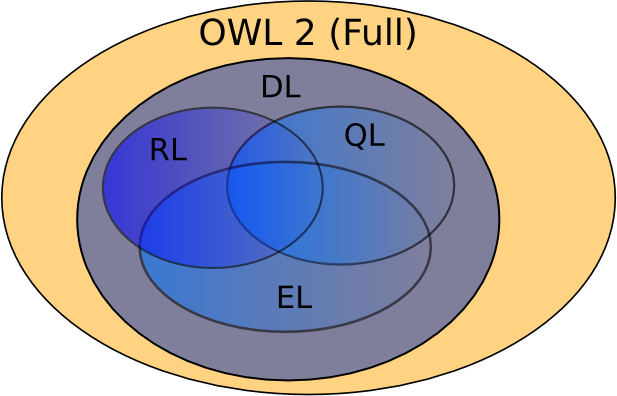
\includegraphics[clip,width=1\columnwidth,bb = 0 0 200 100, draft, type=eps]{/home/john/Desktop/Dissertation/figures/owl2-profiles.png}
\par\end{centering}
\caption{Componentes de um SAD \citet{junior2006sistemas}.\label{fig:Componentes-SAD}}
\end{figure}

A Figura \ref{fig:Componentes-SAD} mostra os componentes genéricos
de um SAD. Eles podem ser divididos em dados, banco de modelos, base
de conhecimento e interface de usuário; o banco de dados armazena
os dados não tratados, é importante que dito banco seja mantido atualizado
para um resultado confiável, o banco de modelos armazena vários modelos
que auxiliam a criação de cenários para a tomada de decisões, o banco
de conhecimento é produzido a partir do entendimento profundo do domínio
de conhecimento no qual são abstraídas as regras do sistema e a interface
de usuário representa cada camada do SADs para que o usuário interaja
com ele.

\section{Arquitetura para Sistemas de Apoio à Decisão}

A arquitetura de um software define a organização em termos de seus
componentes, suas interconexões, suas interações e também suas principais
propriedades \citet{de1997software}. Ela fornece as informações de
como os elementos envolvidos nela se relacionam. Arquiteturas trabalham
a parte externa das ligações entre seus elementos, implementações
internas desses elementos não são considerados arquiteturais \citet{sei2006architecture}.

SADs são criados por especialistas nas áreas de domínio nas quais
eles serão aplicados e implementados por programadores. Esse pode
ser um processo lento e custoso, já que os dois grupos de profissionais
têm \foreignlanguage{english}{\emph{backgrounds}} diferentes e vão
ter problemas de comunicação durante o processo de criação e testes
de um SAD. Esses profissionais podem ser até de organizações diferentes,
o que dificulta ainda mais o processo. Devido ao fato de que os elementos
básicos de todo o SAD (Figura \ref{fig:Componentes-SAD}) serem muito
parecidos, é possível criar uma arquitetura que possa ser re\nobreakdash-usada
em diferentes SADs (ou classes de SADs). Esta arquitetura pode ser
baseada em componentes de software re\nobreakdash-usáveis. Programadores
podem usar essa arquitetura e re\nobreakdash-usar os componentes
de software, já desenvolvidos para ela, para implementar SADs mais
rapidamente.

Para encontrar e configurar componentes de software de uma arquitetura,
uma opção é descrever esses componentes, usando uma ontologia, e usar
os termos dessa ontologia para encontrar os componentes corretos para
uma aplicação \citet{Linhalis2010}. Essas ontologias podem ser criadas
utilizando linguagens padrões da Web Semântica, como a Web Ontology
Language (OWL\nomenclature{OWL}{Web Ontology Language}), para melhor
portabilidade \citet{Pahl2007}. Ontologias e padrões da Web Semântica
serão abordados com mais profundidade no próximo capítulo.

Ontologias, que descrevam componentes de software para serem usados
num SAD de um determinado domínio, terão uma grande quantidade de
termos derivados desse domínio. Especialistas desse domínio terão
familiaridade com esses termos e poderão especificar grande parte
do fluxo de trabalho do SAD usando esses termos. Idealmente, essa
especificação deve ser detalhada o suficiente para que programadores
possam desenvolver a parte computacional do SAD sem necessidade de
mais feedback dos especialistas.

Como especialistas de domínio não têm um conhecimento muito detalhado
sobre linguagens de especificação de sistemas, é necessário o desenvolvimento
de uma \foreignlanguage{english}{Domain Specific Languag}e (DSL) adequada
ao nível de conhecimento de computação dos especialistas. Essa linguagem
também deve conter termos familiares ao domínio desses especialistas. 

\section{Considerações Finais}

Este capítulo apresentou os conceitos principais de SADs, incluindo
a definição geral e a arquitetura de software. Ele também apontou
para a necessidade da geração automática (ou semi\nobreakdash-automática)
de interfaces gráficas de usuários SADs. Uma abordagem para conseguir
a geração automática (ou semi\nobreakdash-automática) de GUIs consiste
na integração com DSLs, onde sejam definidas as características gerais
do sistema e integrado com os conceitos do domínio de conhecimento
a través das ontologias usadas nesses sistemas.
